\documentclass[12pt]{article}
\usepackage[margin=0.5in]{geometry}
\usepackage{graphicx}
\usepackage{alltt}

\begin{document}

\ifx\sevenrm\undefined
  \font\sevenrm=cmr7 scaled \magstep0
\fi

\newread\MyStyle
\openin\MyStyle=src2latex.s2t
\ifeof\MyStyle
  \closein\MyStyle
\else
  \input src2latex.s2t
  \closein\MyStyle
\fi

\ifx\gtfam\undefined
  \ifx\dm\undefined
    \ifx\tendm\undefined
      \def\mc{\null}
    \else
      \def\mc{\tendm}
    \fi
  \else
    \def\mc{\dm}
  \fi
  \ifx\dg\undefined
    \ifx\tendg\undefined
      \def\gt{\null}
    \else
      \def\gt{\tendg}
    \fi
  \else
    \def\gt{\dg}
  \fi
\fi
\ifx\sc\undefined
  \def\sc{\null}
\fi

\tt\mc 

\noindent
\rm\mc {\tt /}{\tt /}\kern0.500em generated\kern0.500em by\kern0.500em Fast\kern0.500em Light\kern0.500em User\kern0.500em Interface\kern0.500em Designer\kern0.500em (fluid)\kern0.500em version\kern0.500em 1.0110

\noindent
\tt\mc \hfill

\noindent
{}{\tt\#}include{\tt\mc \kern0.500em}{\tt "}labfin.h{\tt "}

\noindent
{}\rm\mc {\tt /}{\tt /} \section{Specification} \rm\mc 

\noindent
{\tt /}{\tt /}\kern0.500em This\kern0.500em is\kern0.500em a\kern0.500em soccer\kern0.500em shoting\kern0.500em game.\kern0.500em Players\kern0.500em need\kern0.500em to\kern0.500em shoot\kern0.500em the\kern0.500em ball\kern0.500em without

\noindent
{\tt /}{\tt /}\kern0.500em letting\kern0.500em the\kern0.500em ball\kern0.500em be\kern0.500em captured\kern0.500em by\kern0.500em the\kern0.500em goalie\kern0.500em so\kern0.500em the\kern0.500em player\kern0.500em could\kern0.500em score.

\noindent
{\tt /}{\tt /}\kern0.500em The\kern0.500em goalie\kern0.500em will\kern0.500em move\kern0.500em horizontally\kern0.500em from\kern0.500em left\kern0.500em side\kern0.500em of\kern0.500em the\kern0.500em goal\kern0.500em to\kern0.500em the

\noindent
{\tt /}{\tt /}\kern0.500em right.\kern0.500em Platers\kern0.500em click\kern0.500em the\kern0.500em screen\kern0.500em to\kern0.500em shoot\kern0.500em the\kern0.500em ball.\kern0.500em If\kern0.500em they\kern0.500em miss\kern0.500em the

\noindent
{\tt /}{\tt /}\kern0.500em goal,\kern0.500em the\kern0.500em player\kern0.500em would\kern0.500em have\kern0.500em to\kern0.500em start\kern0.500em over\kern0.500em again.\kern0.500em If\kern0.500em they\kern0.500em score,\kern0.500em 

\noindent
{\tt /}{\tt /}\kern0.500em there\kern0.500em is\kern0.500em a\kern0.500em rank\kern0.500em system\kern0.500em to\kern0.500em cout\kern0.500em their\kern0.500em rank\kern0.500em level.\kern0.500em The\kern0.500em goalie\kern0.500em will\kern0.500em move\kern0.500em 

\noindent
{\tt /}{\tt /}\kern0.500em faster\kern0.500em and\kern0.500em faster\kern0.500em each\kern0.500em time\kern0.500em the\kern0.500em player\kern0.500em scores

\noindent
\tt\mc \hfill

\noindent
{}\rm\mc {\tt /}{\tt /} \clearpage\section{Analysis} \rm\mc 

\noindent
{\tt /}{\tt /}\kern0.500em There\kern0.500em are\kern0.500em two\kern0.500em buttons\kern0.500em on\kern0.500em the\kern0.500em homepage\kern0.500em of\kern0.500em this\kern0.500em game:the\kern0.500em {\tt "}instructions{\tt "}

\noindent
{\tt /}{\tt /}\kern0.500em button\kern0.500em and\kern0.500em the\kern0.500em {\tt "}start{\tt "}\kern0.500em button.\kern0.500em by\kern0.500em clicking\kern0.500em the\kern0.500em {\tt "}instructions{\tt "}\kern0.500em button,

\noindent
{\tt /}{\tt /}\kern0.500em it\kern0.500em willlead\kern0.500em the\kern0.500em player\kern0.500em to\kern0.500em another\kern0.500em window\kern0.500em which\kern0.500em shows\kern0.500em instructions\kern0.500em of

\noindent
{\tt /}{\tt /}\kern0.500em the\kern0.500em game\kern0.500em and\kern0.500em how\kern0.500em to\kern0.500em play\kern0.500em it.\kern0.500em then\kern0.500em they\kern0.500em will\kern0.500em click\kern0.500em the\kern0.500em {\tt "}return{\tt "}\kern0.500em 

\noindent
{\tt /}{\tt /}\kern0.500em button\kern0.500em to\kern0.500em return\kern0.500em to\kern0.500em the\kern0.500em home\kern0.500em screen.\kern0.500em Then\kern0.500em they\kern0.500em click\kern0.500em the\kern0.500em {\tt "}start{\tt "}\kern0.500em 

\noindent
{\tt /}{\tt /}\kern0.500em button\kern0.500em to\kern0.500em start\kern0.500em the\kern0.500em game.\kern0.500em The\kern0.500em player\kern0.500em needs\kern0.500em to\kern0.500em click\kern0.500em on\kern0.500em the\kern0.500em screen

\noindent
{\tt /}{\tt /}\kern0.500em to\kern0.500em shoot\kern0.500em the\kern0.500em ball.\kern0.500em If\kern0.500em they\kern0.500em score,\kern0.500em their\kern0.500em rank\kern0.500em level\kern0.500em will\kern0.500em get\kern0.500em higher.

\noindent
{\tt /}{\tt /}\kern0.500em If\kern0.500em the\kern0.500em goalie\kern0.500em catches\kern0.500em the\kern0.500em ball.\kern0.500em the\kern0.500em rank\kern0.500em level\kern0.500em will\kern0.500em drop\kern0.500em all\kern0.500em the\kern0.500em 

\noindent
{\tt /}{\tt /}\kern0.500em way\kern0.500em down\kern0.500em to\kern0.500em the\kern0.500em beginning\kern0.500em again

\noindent
\tt\mc \hfill

\noindent
{}\rm\mc {\tt /}{\tt /} \clearpage\section{Design} \rm\mc 

\noindent
{\tt /}{\tt /}\kern0.500em  \begin{alltt}
  - The game logo is on top of the home screen.
  - the two buttons are on the left side of the home screen called
  "press start" and "instructions".
  -when you click on "instructions", it will take you to another 
  window which would show the instructions, and there would be a 
  return button to go back to the home screen.
  -the press start button will take you to another window which the 
  game exists.
  -the game window, would have a soccer ball and a goal, and near the 
  goal would be a zombie goalie running left and right.
  \end{alltt}
   \rm\mc 

\noindent
{\tt /}{\tt /} \clearpage\section{Implementation} \rm\mc 

\noindent
\tt\mc {\tt\#}include{\tt\mc \kern0.500em}{\tt <}sstream{\tt >}

\noindent
{}{\tt\#}include{\tt\mc \kern0.500em}{\tt <}iomanip{\tt >}

\noindent
{}{\tt\#}include{\tt\mc \kern0.500em}{\tt <}sys{\tt /}unistd.h{\tt >}

\noindent
{}using{\tt\mc \kern0.500em}namespace{\tt\mc \kern0.500em}std;

\noindent
{}{\tt\#}include{\tt\mc \kern0.500em}{\tt <}FL{\tt /}Fl{\tt\_\kern.141em}GIF{\tt\_\kern.141em}Image.H{\tt >}

\noindent
{}{\tt\#}include{\tt\mc \kern0.500em}{\tt <}FL{\tt /}Fl{\tt\_\kern.141em}JPEG{\tt\_\kern.141em}Image.H{\tt >}

\noindent
{}{\tt\#}include{\tt\mc \kern0.500em}{\tt <}FL{\tt /}Fl{\tt\_\kern.141em}PNG{\tt\_\kern.141em}Image.H{\tt >}

\noindent
{}static{\tt\mc \kern0.500em}const{\tt\mc \kern0.500em}int{\tt\mc \kern0.500em}N1{\tt\mc \kern0.500em}={\tt\mc \kern0.500em}8;{\tt\mc \kern0.500em}\rm\mc {\tt /}{\tt /}\kern0.500em dribble\kern0.500em (intro)

\noindent
\tt\mc static{\tt\mc \kern0.500em}Fl{\tt\_\kern.141em}GIF{\tt\_\kern.141em}Image{\tt *}{\tt\mc \kern0.500em}dribble{\tt\_\kern.141em}images[N1];{\tt\mc \kern0.500em}

\noindent
{}\hfill

\noindent
{}void{\tt\mc \kern0.500em}load{\tt\_\kern.141em}images(){\tt\mc \kern0.500em}{\tt\char'173}

\noindent
{}{\tt\mc \kern1.000em}for(int{\tt\mc \kern0.500em}i=0;{\tt\mc \kern0.500em}i{\tt\mc \kern0.500em}{\tt <}{\tt\mc \kern0.500em}N1;{\tt\mc \kern0.500em}++i)

\noindent
{}{\tt\char'173}

\noindent
{}{\tt\mc \kern0.500em}std::ostringstream{\tt\mc \kern0.500em}oss;{\tt\mc \kern0.500em}oss{\tt\mc \kern0.500em}{\tt <}{\tt <}{\tt\mc \kern0.500em}i;

\noindent
{}{\tt\mc \kern0.500em}std::string{\tt\mc \kern0.500em}s{\tt\mc \kern0.500em}={\tt\mc \kern0.500em}{\tt "}dribble{\tt /}dribble0{\tt "}+oss.str()+{\tt "}.gif{\tt "};

\noindent
{}{\tt\mc \kern0.500em}dribble{\tt\_\kern.141em}images[i]{\tt\mc \kern0.500em}={\tt\mc \kern0.500em}new{\tt\mc \kern0.500em}Fl{\tt\_\kern.141em}GIF{\tt\_\kern.141em}Image(s.c{\tt\_\kern.141em}str());

\noindent
{}{\tt\char'175}

\noindent
{}{\tt\char'175}

\noindent
{}\hfill

\noindent
{}void{\tt\mc \kern0.500em}dribble{\tt\_\kern.141em}animate(void{\tt *}){\tt\mc \kern0.500em}{\tt\char'173}

\noindent
{}{\tt\mc \kern1.000em}static{\tt\mc \kern0.500em}int{\tt\mc \kern0.500em}i{\tt\mc \kern0.500em}={\tt\mc \kern0.500em}0;

\noindent
{}Dribble{\tt -}{\tt >}image(dribble{\tt\_\kern.141em}images[i]);

\noindent
{}i{\tt\mc \kern0.500em}={\tt\mc \kern0.500em}(i{\tt\mc \kern0.500em}+{\tt\mc \kern0.500em}1){\tt\mc \kern0.500em}{\tt\%}{\tt\mc \kern0.500em}N1;

\noindent
{}Dribble{\tt -}{\tt >}parent(){\tt -}{\tt >}redraw();

\noindent
{}double{\tt\mc \kern0.500em}t{\tt\mc \kern0.500em}={\tt\mc \kern0.500em}1.0{\tt /}8;

\noindent
{}Fl::repeat{\tt\_\kern.141em}timeout(t,dribble{\tt\_\kern.141em}animate);

\noindent
{}{\tt\char'175}

\noindent
{}\hfill

\noindent
{}Fl{\tt\_\kern.141em}Double{\tt\_\kern.141em}Window{\tt\mc \kern0.500em}{\tt *}IScreen=(Fl{\tt\_\kern.141em}Double{\tt\_\kern.141em}Window{\tt\mc \kern0.500em}{\tt *})0;

\noindent
{}\hfill

\noindent
{}Fl{\tt\_\kern.141em}Double{\tt\_\kern.141em}Window{\tt\mc \kern0.500em}{\tt *}MainScreen=(Fl{\tt\_\kern.141em}Double{\tt\_\kern.141em}Window{\tt\mc \kern0.500em}{\tt *})0;

\noindent
{}\hfill

\noindent
{}Fl{\tt\_\kern.141em}Box{\tt\mc \kern0.500em}{\tt *}Dribble=(Fl{\tt\_\kern.141em}Box{\tt\mc \kern0.500em}{\tt *})0;

\noindent
{}\hfill

\noindent
{}Fl{\tt\_\kern.141em}Box{\tt\mc \kern0.500em}{\tt *}Gamelogo=(Fl{\tt\_\kern.141em}Box{\tt\mc \kern0.500em}{\tt *})0;

\noindent
{}\hfill

\noindent
{}Fl{\tt\_\kern.141em}Button{\tt\mc \kern0.500em}{\tt *}Instructions=(Fl{\tt\_\kern.141em}Button{\tt\mc \kern0.500em}{\tt *})0;

\noindent
{}\hfill

\noindent
{}static{\tt\mc \kern0.500em}void{\tt\mc \kern0.500em}cb{\tt\_\kern.141em}Instructions(Fl{\tt\_\kern.141em}Button{\tt *},{\tt\mc \kern0.500em}void{\tt *}){\tt\mc \kern0.500em}{\tt\char'173}

\noindent
{}{\tt\mc \kern1.000em}MainScreen{\tt -}{\tt >}hide();

\noindent
{}IScreen{\tt -}{\tt >}show();

\noindent
{}{\tt\char'175}

\noindent
{}\hfill

\noindent
{}Fl{\tt\_\kern.141em}Button{\tt\mc \kern0.500em}{\tt *}Startgame=(Fl{\tt\_\kern.141em}Button{\tt\mc \kern0.500em}{\tt *})0;

\noindent
{}\hfill

\noindent
{}int{\tt\mc \kern0.500em}main(int{\tt\mc \kern0.500em}argc,{\tt\mc \kern0.500em}char{\tt\mc \kern0.500em}{\tt *}{\tt *}argv){\tt\mc \kern0.500em}{\tt\char'173}

\noindent
{}{\tt\mc \kern1.000em}{\tt\char'173}{\tt\mc \kern0.500em}IScreen{\tt\mc \kern0.500em}={\tt\mc \kern0.500em}new{\tt\mc \kern0.500em}Fl{\tt\_\kern.141em}Double{\tt\_\kern.141em}Window(535,{\tt\mc \kern0.500em}500);

\noindent
{}{\tt\mc \kern2.000em}IScreen{\tt -}{\tt >}end();

\noindent
{}{\tt\mc \kern1.000em}{\tt\char'175}{\tt\mc \kern0.500em}\rm\mc {\tt /}{\tt /}\kern0.500em Fl{\tt\_\kern.141em}Double{\tt\_\kern.141em}Window{\tt *}\kern0.500em IScreen

\noindent
\tt\mc {\tt\mc \kern1.000em}{\tt\char'173}{\tt\mc \kern0.500em}MainScreen{\tt\mc \kern0.500em}={\tt\mc \kern0.500em}new{\tt\mc \kern0.500em}Fl{\tt\_\kern.141em}Double{\tt\_\kern.141em}Window(535,{\tt\mc \kern0.500em}500);

\noindent
{}{\tt\mc \kern2.000em}MainScreen{\tt -}{\tt >}color((Fl{\tt\_\kern.141em}Color)FL{\tt\_\kern.141em}GRAY0);

\noindent
{}{\tt\mc \kern2.000em}{\tt\char'173}{\tt\mc \kern0.500em}Dribble{\tt\mc \kern0.500em}={\tt\mc \kern0.500em}new{\tt\mc \kern0.500em}Fl{\tt\_\kern.141em}Box(350,{\tt\mc \kern0.500em}350,{\tt\mc \kern0.500em}74,{\tt\mc \kern0.500em}101);

\noindent
{}{\tt\mc \kern2.000em}{\tt\char'175}{\tt\mc \kern0.500em}\rm\mc {\tt /}{\tt /}\kern0.500em Fl{\tt\_\kern.141em}Box{\tt *}\kern0.500em Dribble

\noindent
\tt\mc {\tt\mc \kern2.000em}{\tt\char'173}{\tt\mc \kern0.500em}Fl{\tt\_\kern.141em}Box{\tt *}{\tt\mc \kern0.500em}o{\tt\mc \kern0.500em}={\tt\mc \kern0.500em}Gamelogo{\tt\mc \kern0.500em}={\tt\mc \kern0.500em}new{\tt\mc \kern0.500em}Fl{\tt\_\kern.141em}Box(125,{\tt\mc \kern0.500em}25,{\tt\mc \kern0.500em}300,{\tt\mc \kern0.500em}180);

\noindent
{}{\tt\mc \kern3.000em}o{\tt -}{\tt >}image(new{\tt\mc \kern0.500em}Fl{\tt\_\kern.141em}PNG{\tt\_\kern.141em}Image({\tt "}gamelogo{\tt /}gamelogo.png{\tt "}));

\noindent
{}{\tt\mc \kern2.000em}{\tt\char'175}{\tt\mc \kern0.500em}\rm\mc {\tt /}{\tt /}\kern0.500em Fl{\tt\_\kern.141em}Box{\tt *}\kern0.500em Gamelogo

\noindent
\tt\mc {\tt\mc \kern2.000em}{\tt\char'173}{\tt\mc \kern0.500em}Fl{\tt\_\kern.141em}Button{\tt *}{\tt\mc \kern0.500em}o{\tt\mc \kern0.500em}={\tt\mc \kern0.500em}Instructions{\tt\mc \kern0.500em}={\tt\mc \kern0.500em}new{\tt\mc \kern0.500em}Fl{\tt\_\kern.141em}Button(100,{\tt\mc \kern0.500em}350,{\tt\mc \kern0.500em}120,{\tt\mc \kern0.500em}40);

\noindent
{}{\tt\mc \kern3.000em}Instructions{\tt -}{\tt >}callback((Fl{\tt\_\kern.141em}Callback{\tt *})cb{\tt\_\kern.141em}Instructions);

\noindent
{}{\tt\mc \kern3.000em}o{\tt -}{\tt >}image(new{\tt\mc \kern0.500em}Fl{\tt\_\kern.141em}JPEG{\tt\_\kern.141em}Image({\tt "}instructions{\tt /}instructions.jpg{\tt "}));

\noindent
{}{\tt\mc \kern2.000em}{\tt\char'175}{\tt\mc \kern0.500em}\rm\mc {\tt /}{\tt /}\kern0.500em Fl{\tt\_\kern.141em}Button{\tt *}\kern0.500em Instructions

\noindent
\tt\mc {\tt\mc \kern2.000em}{\tt\char'173}{\tt\mc \kern0.500em}Fl{\tt\_\kern.141em}Button{\tt *}{\tt\mc \kern0.500em}o{\tt\mc \kern0.500em}={\tt\mc \kern0.500em}Startgame{\tt\mc \kern0.500em}={\tt\mc \kern0.500em}new{\tt\mc \kern0.500em}Fl{\tt\_\kern.141em}Button(100,{\tt\mc \kern0.500em}285,{\tt\mc \kern0.500em}120,{\tt\mc \kern0.500em}40);

\noindent
{}{\tt\mc \kern3.000em}o{\tt -}{\tt >}image(new{\tt\mc \kern0.500em}Fl{\tt\_\kern.141em}JPEG{\tt\_\kern.141em}Image({\tt "}startgame{\tt /}startgame.jpg{\tt "}));

\noindent
{}{\tt\mc \kern2.000em}{\tt\char'175}{\tt\mc \kern0.500em}\rm\mc {\tt /}{\tt /}\kern0.500em Fl{\tt\_\kern.141em}Button{\tt *}\kern0.500em Startgame

\noindent
\tt\mc {\tt\mc \kern2.000em}MainScreen{\tt -}{\tt >}end();

\noindent
{}{\tt\mc \kern1.000em}{\tt\char'175}{\tt\mc \kern0.500em}\rm\mc {\tt /}{\tt /}\kern0.500em Fl{\tt\_\kern.141em}Double{\tt\_\kern.141em}Window{\tt *}\kern0.500em MainScreen

\noindent
\tt\mc {\tt\mc \kern1.000em}IScreen{\tt -}{\tt >}hide();

\noindent
{}load{\tt\_\kern.141em}images();

\noindent
{}Fl::add{\tt\_\kern.141em}timeout(0,dribble{\tt\_\kern.141em}animate);

\noindent
{}{\tt\mc \kern1.000em}MainScreen{\tt -}{\tt >}show(argc,{\tt\mc \kern0.500em}argv);

\noindent
{}{\tt\mc \kern1.000em}return{\tt\mc \kern0.500em}Fl::run();

\noindent
{}{\tt\char'175}

\noindent
{}\rm\mc {\tt /}{\tt /} \clearpage\section{Test} \rm\mc 

\noindent
{\tt /}{\tt /}\kern0.500em  \
  For test, we only need to compile the progam using fltk and open it
  to see if any error has occured. if no error occured, we would do
  ./labfin to see if it has compiled the way we intended it to. 
  and that the things we want there is displaying. The orginal image
  for some reason is not displaying. so i took a screenshot of it.
  \includegraphics{design.png}\\
  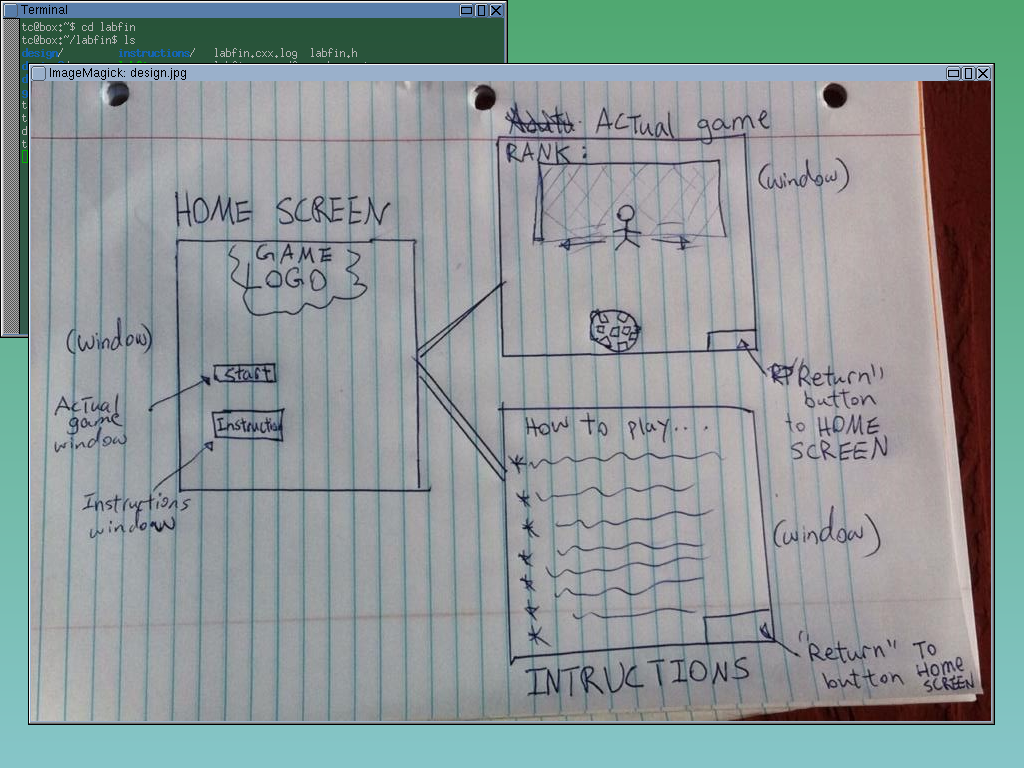
\includegraphics[scale=0.5]{design2.png}\\
   \rm\mc 

\noindent


\rm\mc

\end{document}
